\documentclass[a4paper, 12pt]{report}

\usepackage[utf8]{inputenc}
\usepackage[T1]{fontenc}
\usepackage{lmodern}
\usepackage[ngerman]{babel}
\usepackage[margin=3.0cm,top=4cm]{geometry}
\usepackage[]{graphicx}

\usepackage{array}
\usepackage{lastpage}
\usepackage{blindtext} 
\usepackage{amsmath} 
\usepackage{nicefrac}
\usepackage{float}


\newcolumntype{L}[1]{>{\raggedright\let\newline\\\arraybackslash\hspace{0pt}}m{#1}}
\newcolumntype{C}[1]{>{\centering\let\newline\\\arraybackslash\hspace{0pt}}m{#1}}
\newcolumntype{R}[1]{>{\raggedleft\let\newline\\\arraybackslash\hspace{0pt}}m{#1}}


\usepackage{sectsty}
\sectionfont{\fontsize{15}{15}\selectfont}
\subsectionfont{\fontsize{12}{15}\selectfont}

\renewcommand{\familydefault}{\sfdefault}

\usepackage{fancyhdr}

\pagestyle{fancy}
\fancyhf{}
\fancyhead[L]{Digitale Filter}
\fancyhead[R]{Stefan Urban}
\fancyfoot[R]{Seite \thepage\ von \pageref{LastPage}}
\renewcommand{\headrulewidth}{0.4pt}

%\addtolength{\parskip}{2mm}
\setlength{\parindent}{0pt}


\begin{document}

	\section*{Transformation von p- in z-Ebene}
		\subsection*{Bilineartransformation}
			Prewarping / Vorverzerrung der Grenzfrequenz:
			\[ f'_g = \frac{f_a}{\pi} \cdot \tan \left(\frac{f_x}{f_a}\right) \]
		
			Von der p- in die z-Ebene:
			\[ p\tau = \frac{j\omega}{f_a} = \frac{j2\pi f}{f_a} = 2 \cdot \frac{z - 1}{z + 1} \qquad\qquad \tau = \frac{1}{f_a} \]
			
			Von der z- in die p-Ebende:
			\[ z = \frac{2 + p\tau}{2 - p\tau} \]
		
		\subsection*{Impulsinvariante Transformation}
		Buch: Digitale Filter S.54
		
		\subsection*{Sprunginvariante Transformation}
		Buch: Digitale Filter S.57	
	\vspace{1cm}
	\section*{Nullstellenspiegelung bei MA1-Filtern}
		Liegt die Nullstelle eines MA1-Filters außerhalb des Einheitskreises, kann man über folgende Operation aus einem maximalphasigen Filter $ H(z) $ ein minimalphasiges Filter $ H''(z) $ entwickeln.
		
		Zuerst muss eine Frequenzinversion vorgenommen werden:
		\[ H(z) = 1 + \frac{a}{z} \qquad H'(z) = H\left(\frac{1}{z}\right) = 1 + a\cdot z \]
		
		Da das entstandene Filter akausal ist, muss noch ein Verzögerungsglied eingebaut werden:
		\[ H''(z) = \frac{H'(z)}{z} = a + \frac{1}{z} = a \cdot \left(1 + \frac{1}{a \cdot z}\right) \]
		
		Entstanden ist ein MA1-Filter mit Grundverstärkung $ a $ und Parameter $ \nicefrac{1}{a} $. Der Frequenzgang hat sich dabei nicht geändert!
		
			
\clearpage

	\section*{Linearphasige Filter}
		
		Digitale linearphasige Filter haben ihre Nullstellen in der z-Ebene auf dem oder spiegelsymmetrisch zum Einheitskreis. Pole dürfen nur bei $ z = 0 $ auftreten. Die Gruppenlaufzeit ist frequenzunabhängig.
		\[ \tau_g = \tau \cdot \frac{n}{2} \qquad \tau = \frac{1}{f_a} \]

		Zerlegung der Übertragungsfunktion:
		\[ \underline{H}(w) = H_a(w) \cdot \underline{H}_g(w) = H_a \cdot e^{j\omega\tau_g} \]
		
		Impulsantwort:
		\[ h_0(t) = h_{0a}(t) \ast h{_{0g}}(t) = h_{0a}(t-\tau_g) \]
		
		$ h_{0a}(t) $ ist akausale Impulsantwort, die um die Gruppenlaufzeit $ \tau_g $ verschoben wird, bis die Impulsantwort $ h_0 $ kausal ist.
		
		\subsection*{Erzeugung eines linearphasigen Filters durch Reihenschaltung mit Spiegelfilter}
			
			Das Spiegelfilter besitzt Nullstellen, die zu denen des Ausgangsfilters am Einheitskreis gespiegelt sind. Es darf nur Pole bei $ z = 0 $ erzeugen. Deshalb handelt es sich immer um einen MA2-Filter.
			
			\vspace{0.5cm}
		
			\begin{minipage}[t]{0.5\textwidth}
				Filter:
				
				\begin{figure}[H]
					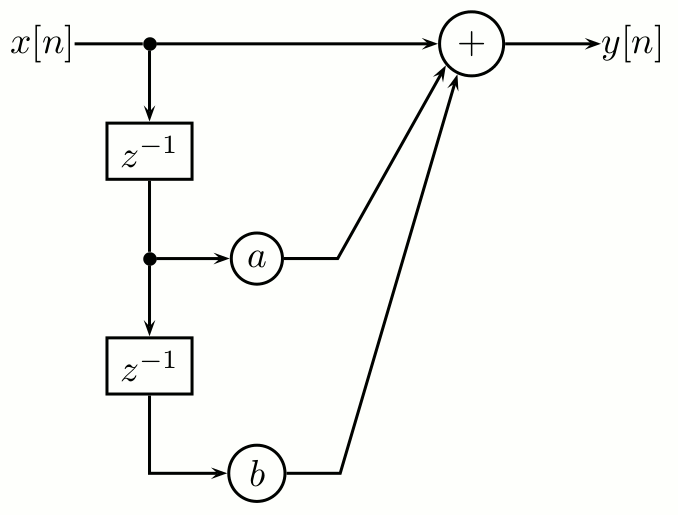
\includegraphics[width=\textwidth]{images/ma2_ab.png}
				\end{figure}
			\end{minipage}
			\begin{minipage}[t]{0.5\textwidth}
				Spiegelfilter
				
				\vspace{-0.1cm}
				
				\begin{figure}[H]
					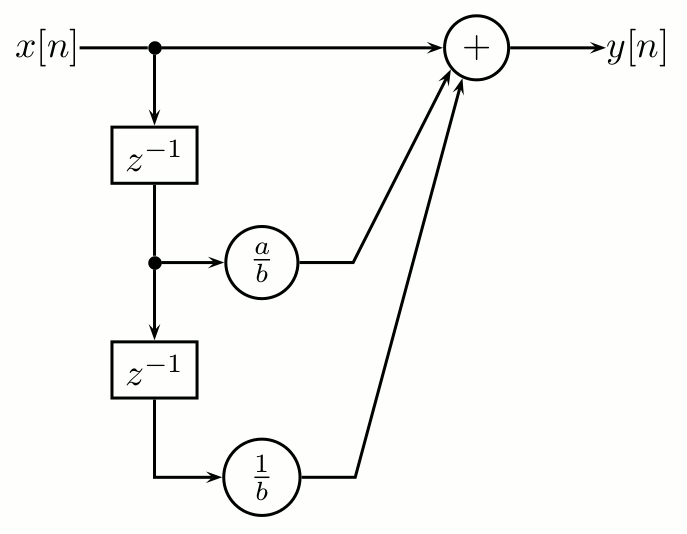
\includegraphics[width=\textwidth]{images/ma2_ab_spiegel.png}
				\end{figure}
			\end{minipage}
			
			\vspace{0.5cm}
			
			Berechnung:
			
			Die Nullstellen des Spiegelfilters werden bestimmt über den Nullstellenradius und den Winkel. Der Nullstellenradius ist der reziproke Nullstellenradius der Ausgangsfilters. Die Winkel bleiben gleich (genau genommen werden sie negiert, was sich aber egalisiert).
			
			\[ R_0 = \frac{1}{\sqrt{b}} \qquad \Longrightarrow \qquad R_{0,neu} = \frac{1}{R_0} = \frac{1}{\sqrt{\frac{1}{b}}} \Longrightarrow b_{neu} = \frac{1}{b} \]
			
\clearpage

	\section*{Kombinationen}
		\begin{minipage}[t]{0.5\textwidth}
			\subsection*{Parallelschaltung}
				\[ H_{ges}(z) = H_1(z) + H_2(z) \]
		\end{minipage}
		\begin{minipage}[t]{0.5\textwidth}
			\subsection*{Serienschaltung}
				\[ H_{ges}(z) = H_1(z) \cdot H_2(z) \]
		\end{minipage}
		
		\vspace{0.5cm}

		\begin{minipage}[t]{0.5\textwidth}
			\subsection*{Rückkopplung}
				\[ H_{ges} = \frac{H_1(z)}{1 - H_1(z) \cdot H_2(z)} \]
		\end{minipage}
		\begin{minipage}[t]{0.5\textwidth}
			\vspace{-0.3cm}
			\begin{figure}[H]
				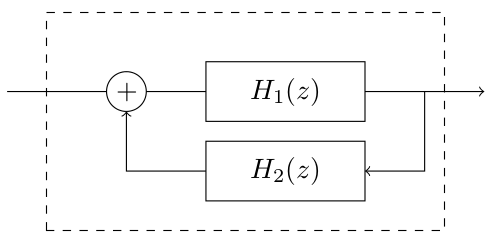
\includegraphics[width=0.6\textwidth]{images/digitale_filter_rueckkopplung.png}
			\end{figure}
		\end{minipage}
		
		\vspace{-0.3cm}
		
		\subsection*{Allpass 1. Ordnung}
		
		\vspace{-0.8cm}
			
			\begin{minipage}[t]{0.5\textwidth}
				\begin{figure}[H]
					\centering
					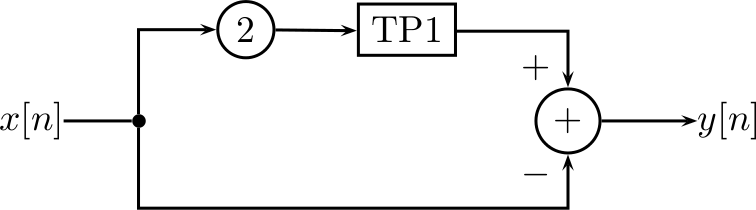
\includegraphics[width=0.9\textwidth]{images/parallel_ap1_1.png}
				\end{figure}
				\begin{center}
					AP1 (Typ 1)
				\end{center}
			\end{minipage}
			\begin{minipage}[t]{0.5\textwidth}
				\begin{figure}[H]
					\centering
					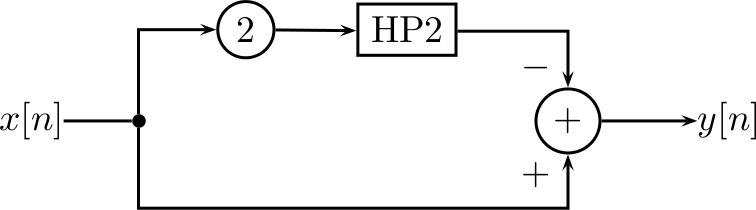
\includegraphics[width=0.9\textwidth]{images/parallel_ap1_2.png}
				\end{figure}
				\begin{center}
					AP1 (Typ 2)
				\end{center}
			\end{minipage}
			
		\subsection*{Allpass 2. Ordnung}
		\vspace{-0.8cm}
			
			\begin{minipage}[t]{0.5\textwidth}
				\begin{figure}[H]
					\centering
					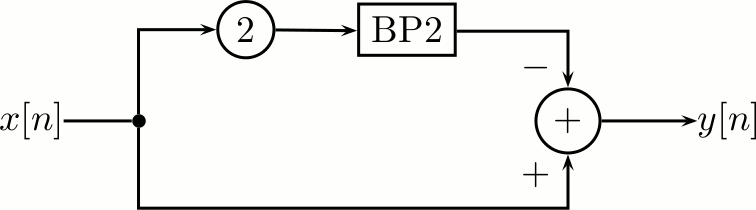
\includegraphics[width=0.9\textwidth]{images/parallel_ap2_1.png}
				\end{figure}
				\begin{center}
					AP2 (Typ 1)
				\end{center}
			\end{minipage}
			\begin{minipage}[t]{0.5\textwidth}
				\begin{figure}[H]
					\centering
					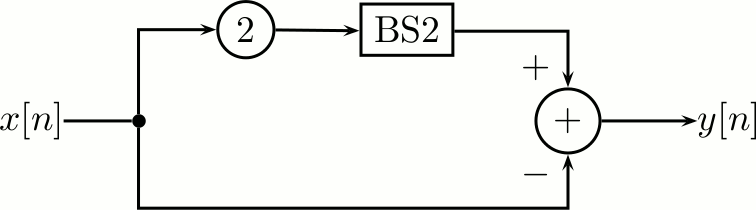
\includegraphics[width=0.9\textwidth]{images/parallel_ap2_2.png}
				\end{figure}
				\begin{center}
					AP2 (Typ 2)
				\end{center}
			\end{minipage}
			
			
		\subsection*{Tief- und Hochpass 1. Ordnung}
		\vspace{-0.8cm}
			
			\begin{minipage}[t]{0.5\textwidth}
				\begin{figure}[H]
					\centering
					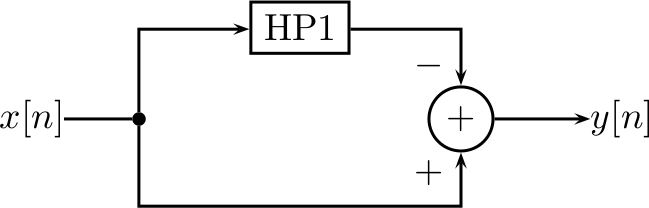
\includegraphics[width=0.9\textwidth]{images/parallel_tp1.png}
				\end{figure}
				\begin{center}
					TP1
				\end{center}
			\end{minipage}
			\begin{minipage}[t]{0.5\textwidth}
				\begin{figure}[H]
					\centering
					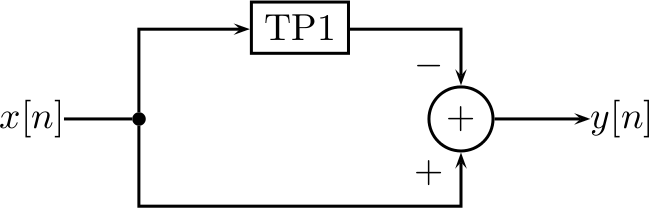
\includegraphics[width=0.9\textwidth]{images/parallel_hp1.png}
				\end{figure}
				\begin{center}
					HP1
				\end{center}
			\end{minipage}
			
		\subsection*{Equalizer 2. Ordnung}
		\vspace{-0.5cm}
			\begin{figure}[H]
				\centering
				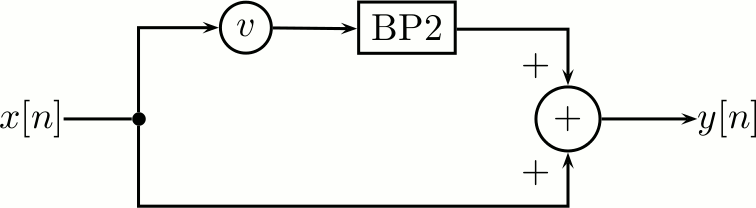
\includegraphics[width=0.45\textwidth]{images/parallel_eq2.png}
			\end{figure}
			\begin{center}
				EQ2
			\end{center}
		
\clearpage

	\section*{Symmetrische und antimetrische Filter}
		
		Ein symmetrischer Filter n-ter Ordnung kann in ein symmetrisches und ein antimetrisches Filter mit jeweils der halben Ordnung aufgeteilt werden.

\end{document}
